\documentclass{paris17}
\usepackage{amsmath}
\usepackage{graphicx}
\usepackage{graphicx}
\usepackage{caption}
\usepackage{subcaption}
\usepackage{floatrow}
% Table float box with bottom caption, box width adjusted to content
\newfloatcommand{capbtabbox}{table}[][\FBwidth]
\usepackage{capt-of}% or \usepackage{caption}
\usepackage{booktabs}
\usepackage{varwidth}


\begin{document}

\section{Introduction}

Propagating wavefields using the explicit finite difference method is the kernel of reverse time migration (RTM) and high-end velocity algorithms in seismic applications. In recent decades there has been a significant increase of interest in the seismic exploration community to invert the image of the subsurface in larger regions and higher resolutions in the elastic media, which brings tremendous computing challenges. As a result, the optimizing methods for improving the performance of the wavefield propagation are in great demands.

One approach to improving the performance of modeling is to recognize that the Earth attenuates seismic energy. We can ignore higher and higher frequencies and still obtain an accurate image\cite[]{Clapp.sep.111.bob3} when we push the wavefield down in depth. By using coarser sampling at large time steps based on the stability and dispersion conditions, we can reduce the computational cost for wavefield propagation. 

The concept of the constant-Q model introduced by \cite{Kjartansson.sep.23} is used to approximate the attenuation. However, the formulation for computing the time derivative of the constant-Q model requires to store wavefields from previous values to present time, which is impractical for real seismic modeling in terms of memory capacities on modern computers. Zhu developed a constant-Q wave equation using fractional Laplacian operators which avoid the need for storing the past values of the wavefields \cite[]{zhu2014theory,shen2013wave}. However, the proposed method is for the 2D viscoelastic case and the computational cost of fractional Laplacian is still expensive compared with the conventional Laplacian.

Meanwhile, the Nvidia Graphic Processing Units (GPUs)  have achieved a great success in many domains. In seismic applications, GPUs are employed as high-performance computing accelerators for key seismic modeling, imaging and inversion kernels due to their high memory bandwidth and a large number of processing units \cite[]{he2015gpu}.

This work proposes a high performance design of accelerating the wavefield propagation in 3D elastic media by approximating the constant Q propagation on multiple Nvidia GPUs. We first propose the Q approximation formulation by extending the formulation from the 2D viscoelastic to the 3D viscoelastic case where the fractional Laplacian is approximated to the conventional Laplacian and the dispersion term is ignored.  Optimization strategies from different aspects (memory, occupancy, and overlapping) are performed to form an efficient kernel on multiple GPUs. To further improve the performance, a set of tricks are also applied to reduce the computation. Combining all the optimization schemes, we can achieve a significant speedup of 60 to 200 times over a highly optimized 24-core CPU solution for the 3D elastic wavefield propagation.

\section{Method and Theory}

\subsection{Constant Q formulation}

Our theory is built on the foundation of \cite{zhu2014theory}. The time-domain differential equation is based on the Laplacian differential operators of fractional order, which is able to model seismic wave propagation in constant-Q viscoelastic media. The stress-strain relation is derived from the classical equation expressed in terms of fractional time derivatives. The formulation has the advantage of not requiring additional field variables so that it saves the computing time and storage significantly.

We extend the formulation of \cite{zhu2014theory} from the 2D viscoelastic case to the 3D viscoelastic case. Note that the Laplacian differential operators of fractional order bring extra computational costs to the elastic modeling, we approximate it with the conventional Laplacian operators, which not only significantly reduces the computing complexities but also preserves the accuracy if Q is not extremely low \cite[]{shen2015image}. We further reduce the computational costs by ignoring the dispersion terms because it makes little effects compared with the attenuation of the signals. As a result, our equations are as follows.

\begin{equation}
\begin{bmatrix} \sigma_{11}\\ \sigma_{22}\\ \sigma_{33} \end{bmatrix} = \begin{bmatrix} \frac{\partial \tau_p^{(1)}}{\partial t} + c_{11} & \frac{\partial \tau_p^{(1)}}{\partial t} - 2\frac{\partial \tau_s^{(1)}}{\partial t} +c_{12}& \frac{\partial \tau_p^{(1)}}{\partial t} - 2\frac{\partial \tau_s^{(1)}}{\partial t} +c_{13} \\ \frac{\partial \tau_p^{(2)}}{\partial t} - 2\frac{\partial \tau_s^{(2)}}{\partial t} +c_{12}& \frac{\partial \tau_p^{(2)}}{\partial t} + c_{22} & \frac{\partial \tau_p^{(2)}}{\partial t} - 2\frac{\partial \tau_s^{(2)}}{\partial t} +c_{23}\\ \frac{\partial \tau_p^{(3)}}{\partial t} - 2\frac{\partial \tau_s^{(3)}}{\partial t} +c_{13} & \frac{\partial \tau_p^{(3)}}{\partial t} - 2\frac{\partial \tau_s^{(3)}}{\partial t} +c_{23} & \frac{\partial \tau_p^{(3)}}{\partial t} + c_{33} \end{bmatrix} \begin{bmatrix} \epsilon_{11}\\ \epsilon_{22}\\ \epsilon_{33} \end{bmatrix}
\end{equation}

\begin{equation}
  \sigma_{12} = \left ( 2\frac{\partial}{\partial t} \left( \frac{c_{11}-c_{12}}{2}c_s^{(2\gamma_s-1)}\sin(\pi\gamma_s) \right) + c_{66} \right )\times \epsilon_{12}
\end{equation}

\begin{equation}
  \sigma_{13} = \left ( 2\frac{\partial}{\partial t} \left( \frac{c_{33}-c_{13}}{2}c_s^{(2\gamma_s-1)}\sin(\pi\gamma_s) \right) + c_{55} \right )\times \epsilon_{13}
\end{equation}

\begin{equation}
  \sigma_{23} = \left ( 2\frac{\partial}{\partial t} \left( \frac{c_{22}-c_{23}}{2}c_s^{(2\gamma_s-1)}\sin(\pi\gamma_s) \right) + c_{44} \right )\times \epsilon_{23}
\end{equation}

\begin{equation}
  \tau_p^{(1)} = c_{11}C_p^{2\gamma_p - 1}\sin(\pi \gamma_p)
\end{equation}

\begin{equation}
  \tau_s^{(1)} = \frac{c_{11} - c_{13}}{2}C_s^{2\gamma_s - 1}\sin(\pi \gamma_s)
\end{equation}

\begin{equation}
  \gamma_{p,s}=\frac{1}{\pi}\tan^{-1}(\frac{1}{Q_{p,s}})
\end{equation}

where $\sigma$ is the stress tensor; $\epsilon$ is the strain tensor; $c_{ij}$ is the forth-order stiffness tensor; $C_p$ and $C_s$ are the velocities of P-wave and S-wave. $Q_{p,s}$ is the constant factor for the attenuation of P-wave and S-wave, respectively. Note that we only present how $\tau_p^{(1)}$ and $\tau_s^{(1)}$ are derived$. \tau_p^{(2)}$,$\tau_p^{(3)}$, $\tau_s^{(2)}$ and $\tau_s^{(3)}$ can be derived in a similar way.

The reasons why our constant Q formulation is relatively computationally economic are as follows. (1) The fractional Laplacian is approximated to the conventional Laplacian. (2) The dispersion term is ignored. (3) We preserve the original workflow of elastic modeling while only adding a few terms when computing stress tensors from train tensors.

\subsection{GPU Optimizations}

The reason why GPUs outperform CPUs significantly on many scenarios is that the architecture of GPUs favors the throughput of many data-parallel tasks over the latency of a single thread. We have an efficient parallel design on the multiple-GPU platform with three main strategies.

Firstly, we fully utilize the hierarchical memory of the GPU. We keep a set of constant variables such as the derivative coefficients in the constant memory and the read-only cache. As the 64KB first-level cache can be configured as different combinations between L1 cache and shared memory, we configure it dynamically in different scenarios. For the 8th-order stencil computation, we configure the first-level cache by setting the sizes of shared memory and L1 cache to 48 KB and 16 KB, respectively, which achieves great performance based on the 3D stencil design proposed by \cite{micikevicius20093d}. For others, we prefer to configure the first-level cache as the L1 cache where we don't use shared memory explicitly.

Secondly, we carefully tune the number of registers per thread to maximize the occupancy of GPUs. Since the access pattern of GPU global memory in the stencil kernel is irregular, the more threads there are, the less latency it gains for memory access. However, as the number of registers is limited in a streaming multiprocessor (SM), increasing the number of registers per thread will decrease the number of active warps. So it is important to have a strategy to balance them. We first remove the intermediate variables to reduce the number of registers per thread. Then we dynamically track the performance by adjusting the block size and the \emph{maxrregcount} compiler option.

Thirdly, we design a computation and communication overlapping scheme to maximize the utilization of different kinds of resources. The entire wavefield domain is divided into 4 subdomains, each assigning to a GPU shown in Figure \ref{fig:domain-decomposition}. Note that we need ghost cells to store and exchange the halos, which is denoted by the arrows. In each subdomain, we further divide it into three parts, the halo part, the outer part and the inner part as shown in Figure \ref{fig:task-decomposition}. The computation of inner and outer parts is assigned to different CUDA streams so that they are executed concurrently. When the computation of the outer part is finished, the GPU starts exchanging halos with its neighbors. In this way, the computation of the inner part can hide the communication time perfectly, shown in Figure \ref{fig:overlap}.

\begin{figure}[h]
    \centering
    \begin{subfigure}[b]{0.3\textwidth}
        \centering
        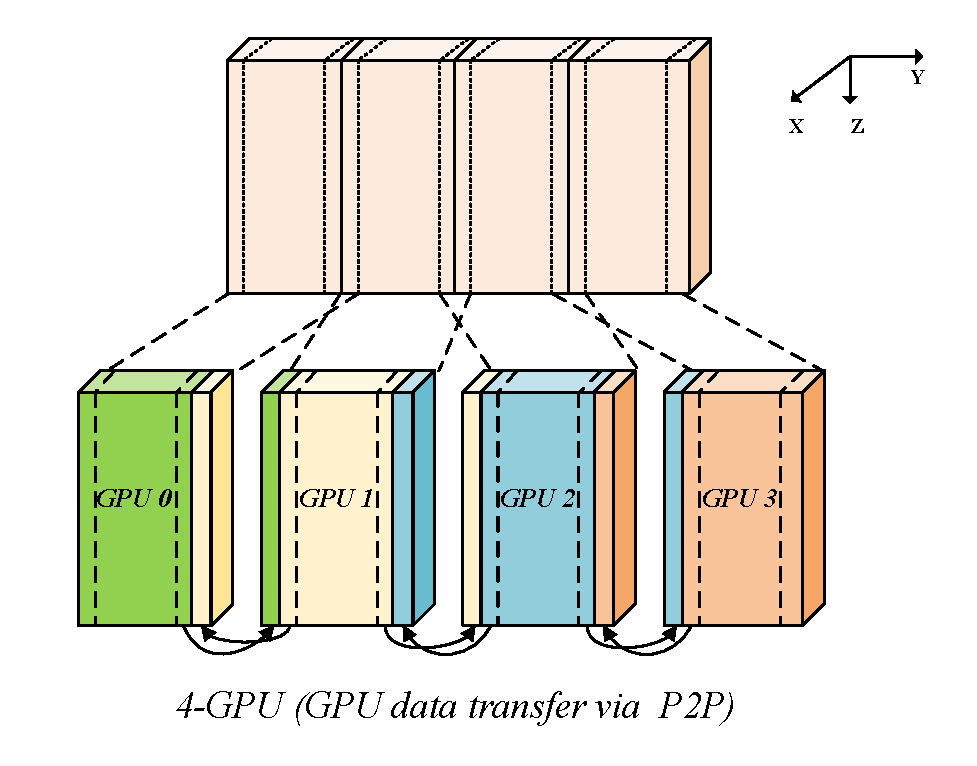
\includegraphics[height=1.3in]{./fig/domain-decompose.pdf}
        \caption{Domain decomposition}
        \label{fig:domain-decomposition}
    \end{subfigure}%
    ~
    \begin{subfigure}[b]{0.3\textwidth}
        \centering
        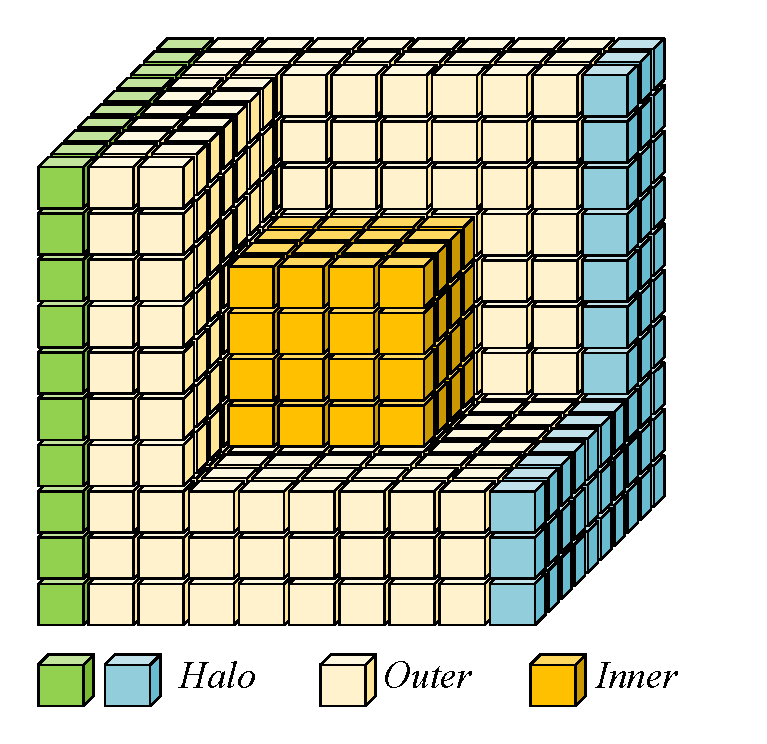
\includegraphics[height=1.3in]{./fig/inner-outer.pdf}
        \caption{Task decomposition}
        \label{fig:task-decomposition}
    \end{subfigure}
    ~
    \begin{subfigure}[b]{0.3\textwidth}
        \centering
        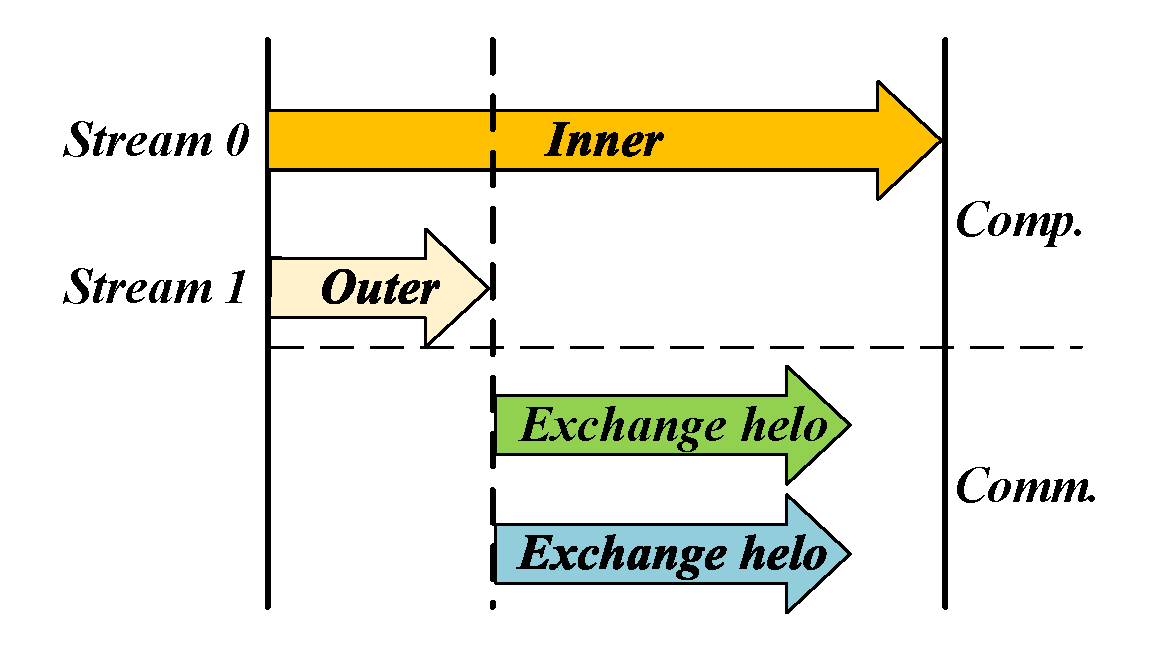
\includegraphics[height=1.1in]{./fig/overlap.pdf}
        \caption{Comp. \& Comm. overlapping}
        \label{fig:overlap}
    \end{subfigure}
    \caption{Computation and communication overlapping over multiple GPUs.}
\end{figure}

\subsection{Other Optimization Tricks}

Apart from the GPU-based optimization, we also apply another two approaches to further improve the performance.  (1) After taking the energy attenuation into consideration, we can ignore the frequencies that have attenuated. Therefore, the grid cells and the time steps can get larger as the wavefields propagate in time. We can achieve significant speedup when we resample the velocities and wavefields to coarser grids, especially in longer time steps. Using the above approach, the early time steps dominate the computation. (2) We eliminate the bottleneck by applying another trick that it is not necessary to propagate the wavefields significantly away from the source at early times. So the update of the wavefields where the waves have not reached so far is eliminated.



\section{Experiments}

\subsection{Q Effects}
Experiments for demonstrating the functionality of applying the Q effect and the performance with different optimization strategies are presented. Figure \ref{fig:with-attenuation} shows the z-x plane of the z-component of the 3D wavefield using standard elastic wave equation at 0.9 seconds while Figure \ref{fig:without-attenuation} shows the wavefields with the constant Q ($Q_s=Q_p=20$) added at the same time step. We can observe that the wavefields are nearly identical except that the wavefront in Figure \ref{fig:with-attenuation} is weaker, which is reasonable owning to the energy attenuation. The spectrums of the wavefields give a better illustration for the attenuation, which is shown in Figure \ref{fig:spectrum}.

\begin{figure}[h]
    \centering
    \begin{subfigure}[b]{0.3\textwidth}
        \centering
        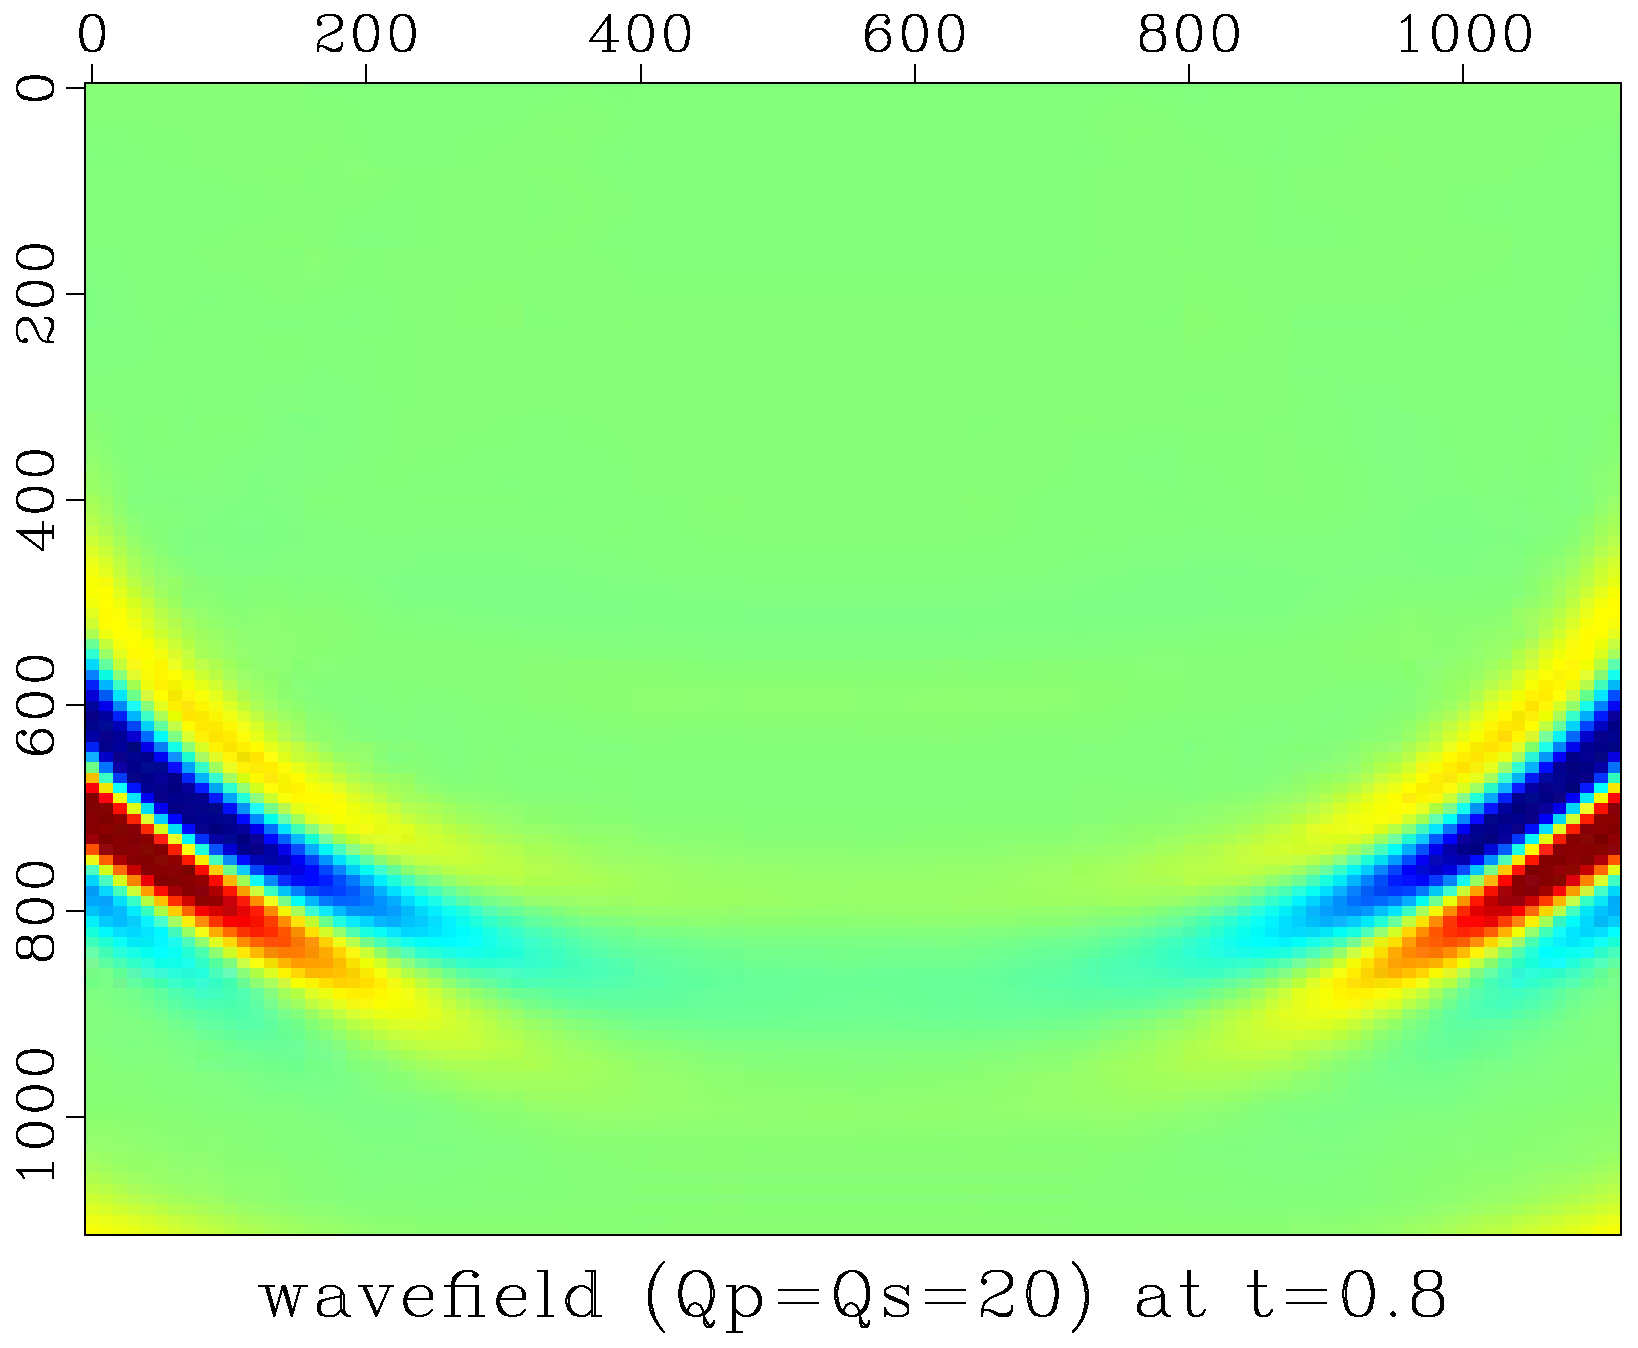
\includegraphics[height=1.3in]{./fig/q20.pdf}
        \caption{Wavefield with attenuation}
        \label{fig:with-attenuation}
    \end{subfigure}
    ~
    \begin{subfigure}[b]{0.3\textwidth}
        \centering
        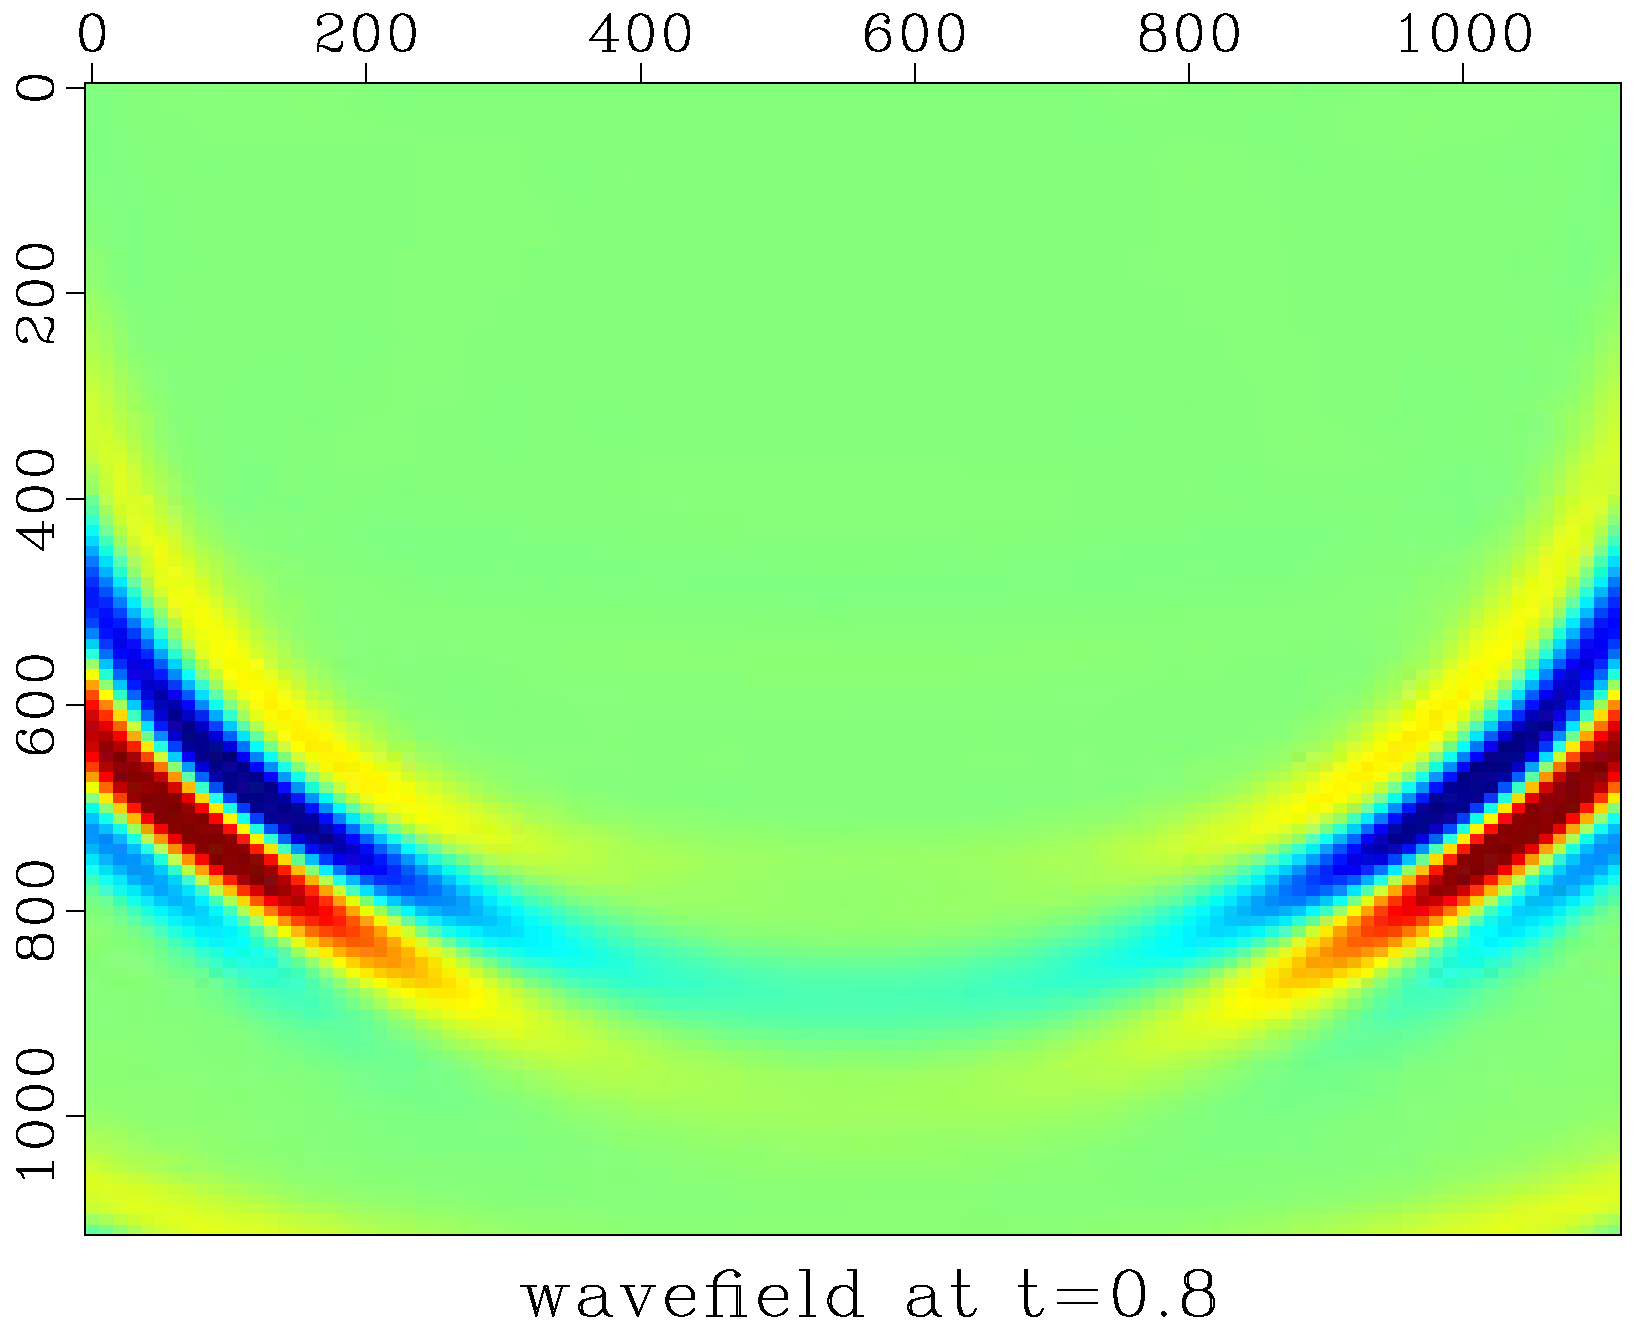
\includegraphics[height=1.3in]{./fig/std.pdf}
        \caption{Wavefield without attenuation}
        \label{fig:without-attenuation}
    \end{subfigure}%
    ~
    \begin{subfigure}[b]{0.3\textwidth}
        \centering
        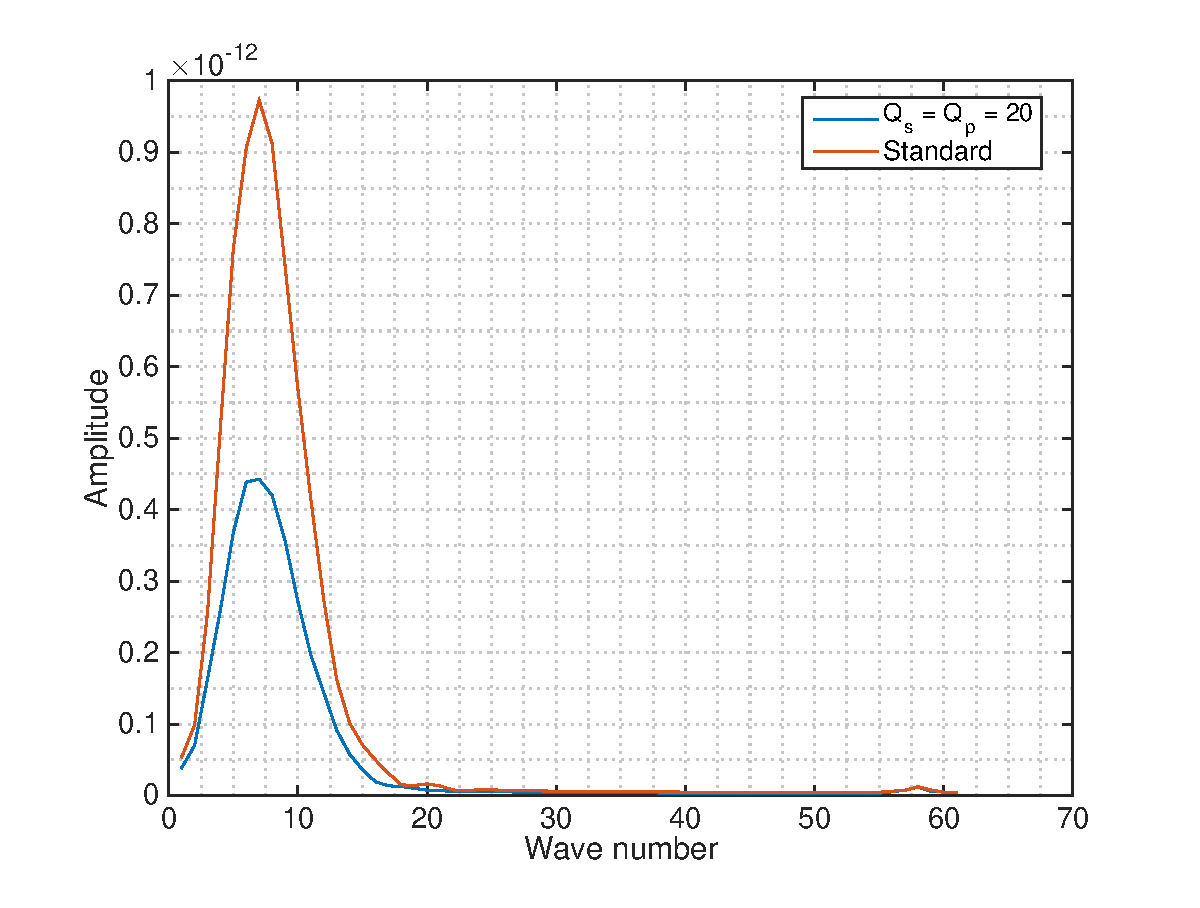
\includegraphics[height=1.3in]{./fig/spec.eps}
        \caption{Spectrum of the wavefields}
        \label{fig:spectrum}
    \end{subfigure}
    \caption{Wavefields with and without attenuation.}
\end{figure}

\subsection{Performance}

We propagate the wavefield in the 3D domain of size $700\times700\times700$ for 6000 time steps to measure the performance. Figure \ref{fig:gpu-speedup} shows the performance speedup of 1-4 K40 GPUs over one 24-core CPU node. The GPU design among 4 K40 GPUs can significantly improve the performance of the computational part by 96 times, and improve the overall performance by 63 times. Note that the CPU design is also well tuned by using multi-threading and vectorization. Figure \ref{fig:q-speedup} shows the speedup as a function of propagation time for different Q values. We can see that we obtain a great performance gain at the early and late time steps because we restrict the computing region at the early time steps and ignore the high frequencies at the late time steps. The longer the time records, the more significant speedup we achieve. Combining all optimization schemes as well as the GPU-based optimizations, we can achieve a performance speedup of 60x to 200x as a function of Q.

\begin{figure}[h]
    \centering
    \begin{subfigure}[b]{0.4\textwidth}
        \centering
        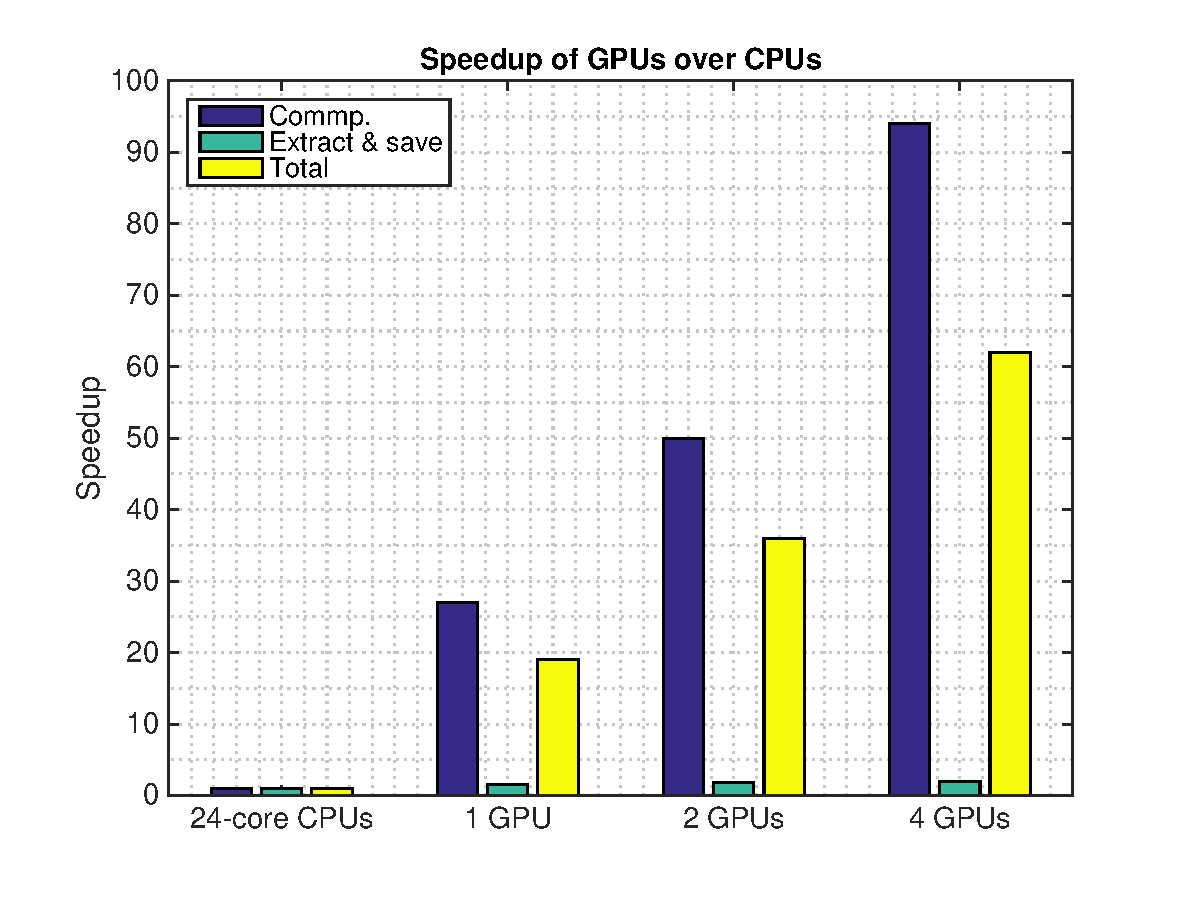
\includegraphics[height=1.5in]{./fig/speedup.eps}
        \caption{Speedup with GPU optimizations}
        \label{fig:gpu-speedup}
    \end{subfigure}%
    ~
    \begin{subfigure}[b]{0.4\textwidth}
        \centering
        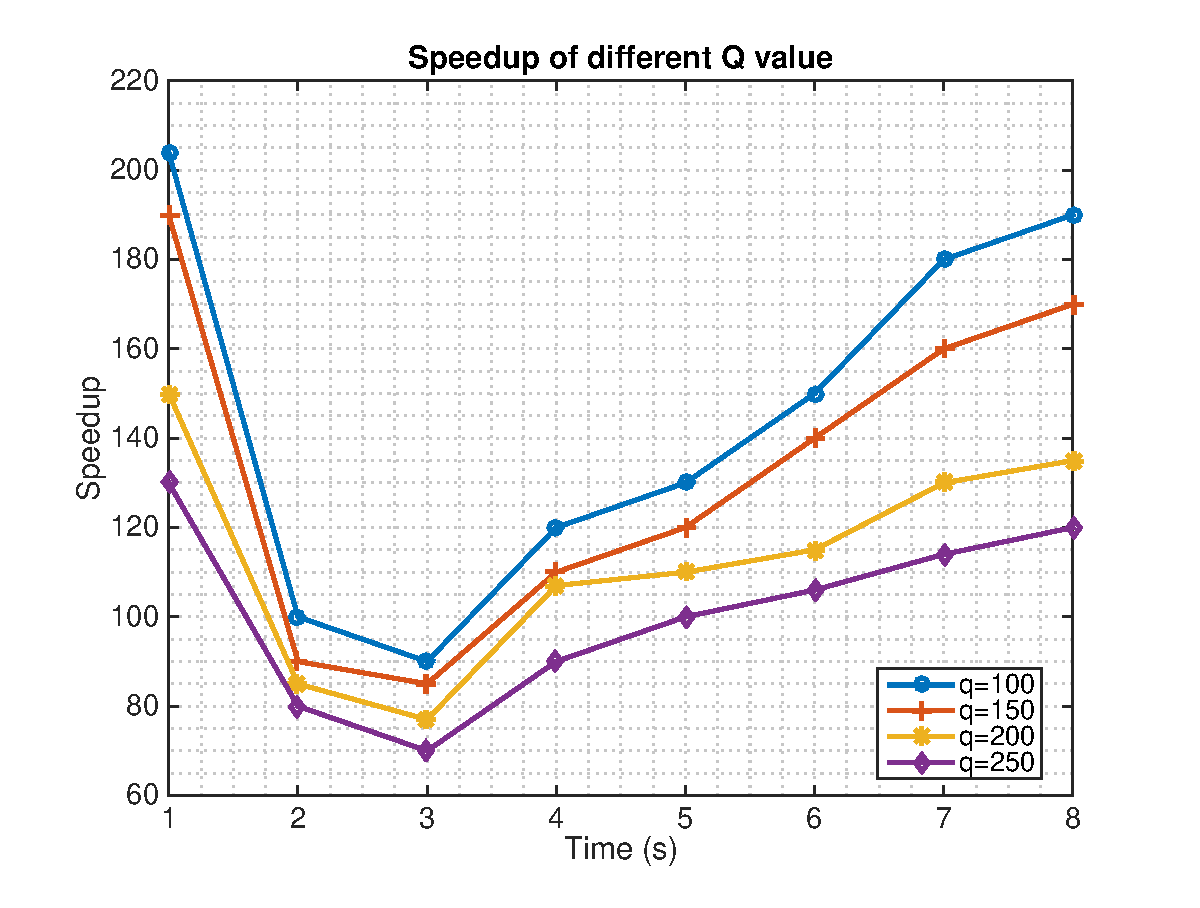
\includegraphics[height=1.5in]{./fig/speedup_q.eps}
        \caption{Speedup as different Q value}
        \label{fig:q-speedup}
    \end{subfigure}
    \caption{Performance results of GPU optimizations and energy attenuation}
\end{figure}

\section{Conclusions}

This work manages to boost the performance of the wavefield propagation in 3D elastic scenarios by approximating the Q propagation and using the multi-GPU platform. We first extend the constant-Q formulation from the 2D viscoelastic case to the 3D viscoelastic case. Different optimization techniques on GPUs are then described for an efficient modeling kernel. We also propose a set of schemes to reduce the computation to further improve the performance. The experimental results show that we can achieve significant performance speedups of 60 to 200 times with 4 GPUs over the CPU-based solution as a function of Q.

\bibliography{bob}

\end{document}

